\documentclass[titlepage]{article}


\usepackage{graphicx} % Required for inserting images
\usepackage{array}
\usepackage{tikz}
\usepackage{tabularx}
\usepackage{float}

\usepackage{hyperref}
\hypersetup{
    colorlinks=true,
    citecolor=black,
    linkcolor=black,
    urlcolor=blue
}
\usepackage{biblatex}
\addbibresource{reference.bib}
\title{Project Proposal: Process Behavior Analysis with Focused Clustering}
\author{Isaac Amann}
\date {12/13/2023}




\newcommand{\requirementTable}[6]{
\begin{center}
    \begin{tabularx}{\textwidth}{| X | X | X |}
    \hline
    \multicolumn{3}{|l|}{\textbf{#1}} \\
     \hline
     \multicolumn{3}{|l|}{#2}\\
     \hline
     \multicolumn{3}{|l|}{Origin: #3} \\
     \hline
     Version: #4 & Date: #5 & Priority: #6\\
     \hline
    \end{tabularx}
\end{center}
}
\newcommand{\requirement}[7]
{
        \begin{table}[H]
            \centering
            \begin{tabular}{|@{}p{\textwidth}@{}|}
                \hline
                \textbf{#1} \\
                \hline
                Goal: #2 \\
                \hline
                #3 \\
                \hline
                Origin: #4 \\
                \hline
                \begin{tabular}{c|c|c}
                    Version: #5 & Date: #6 & Priority: #7\\
                \end{tabular}\\
            \hline
            \end{tabular}
        \end{table}
}

\newcommand{\longUseCase}[3]
{
    \def\tempMainFlow{#1}%
    \def\tempExtension{#2}%
    \usecase#3
}

\newcommand{\usecase}[9]
{
    \begin{table}[H]
        \centering
        \begin{tabularx}{\textwidth}{|X | X|}
        \hline
            \textbf{Use Case Name} & #1\\
        \hline
            \textbf{Related Requirements} & #2\\
        \hline
            \textbf{Goal In Context} & #3\\
        \hline
            \textbf{Preconditions} & #4\\
        \hline
            \textbf{Successful End Condition} & #5\\
        \hline
            \textbf{Failed End Condition} & #6\\
        \hline
            \textbf{Primary Actors} & #7\\
        \hline
            \textbf{Secondary Actors} & #8\\
        \hline
            \textbf{Trigger} & #9\\
        \hline
            \textbf{Main Flow} & \tempMainFlow\\
        \hline
            \textbf{Extensions} & \tempExtension\\
        \hline
        \end{tabularx}
    \end{table}
    
}



\begin{document}

\maketitle
\tableofcontents

\section{Abstract}
\begin{flushleft}
    Windows programs have to use Windows API functions in order to interact with the operating system. These are often abstracted through the use of libraries, but programs still use them even if the programmer does not interact with them directly \cite{winAPI}. By counting the API calls made by processes, a data set can be created where process behavior can be analyzed. A motivating example of this would be ransomware. Ransomware programs would make many file access API calls since most files on the system would be opened in order to encrypt them. Other programs with a similar number of file access API calls may also be ransomware. In a large enough data set, it may be possible to group programs by their behavior.
\end{flushleft}

\section{Introduction}
\begin{flushleft}
Windows applications interface with the Windows operating system through a series of API calls found within DLL files on the system. A process's behavior could be modeled as a data point consisting of the total of times a process made a specific API call during execution for each API call monitored by the system. The system will use DLL injection to overwrite the addresses of Windows API calls in the target process's memory. The functions overwriting the default functions will include code for counting API calls made before redirecting to the original call. The data set created by this system can then be analyzed by different data analysis techniques including clustering and focused clustering. 
\end{flushleft}

\begin{flushleft}
Initially I planned on using the C++ library Detours released by Microsoft in order to reroute API calls. The library contains functions for attaching to specific API calls and altering their behavior \cite{detours}. The library included the functionality needed, but could only attach to processes at start of execution and not into already running processes. To attach to an already running process, a remote thread should be opened on the target process where loadLibrary can be called in order to inject a DLL that will overwrite the monitored API calls in the target process's memory \cite{hookingSample}. This technique should not disrupt a process since it is only inserting a small operation that should be executed before calling the original API call, but testing will be required to ensure it does not make programs unstable. The article showing this technique was posted in 2002, but everything used is still present in the Windows API documentation from Microsoft so it should still be viable.
\end{flushleft}

\begin{flushleft}
The main data analysis technique used by the system will be focused clustering using the Sow And Grow algorithm currently being developed by Dr. Che. The algorithm is based on DBSCAN but instead of clustering the entire data set, certain data points are passed as seed points. The algorithm then uses this seed points to grow clusters around them. Processes of interest will be used as seed points to grow clusters in the data set that should contain data points corresponding to processes with similar behavior to that of the processes used as seed points.
\end{flushleft}
\begin{flushleft}
    The main motivation for doing this is malware detection. A known sample of a specific type of malware could be used as a seed point and processes that happen to fall into the cluster grow from this seed point may be malware of the same type. Using this method, malware in the data set that has eluded other detection methods could be revealed. 
\end{flushleft}

\begin{flushleft}
    Version control will be done through Github. The following repositories will be used.\\
    Collection Server: \url{https://github.com/IsaacAmann/Windows-API-Monitor-Collection-Server}\\
    Collection Client: \url{https://github.com/IsaacAmann/Windows-API-Monitor}
\end{flushleft}

\section{Requirements}


\subsection{Collection Methods}
Requirements were collected over multiple meetings with Dr. Che and other students working on the Sow And Grow research project. Requirements were also collected while working on an early prototype.
\subsection{Functional Requirements}


\requirement
{FR1 Server Data Collection}
{Collection Server should collect Data Points from Client }
{Collection Server should host an API endpoint that allows Client software to send Data Points collected while monitoring processes on the host system}
{}{1.0}{11/01/2023}{high}

\requirement
{FR2 Client Side Data Collection}
{Client software should monitor running processes}
{Client should monitor processes running on the host system and collect Data Points that include the number of Windows API calls made by the processes.}
{}{1.0}{11/01/2023}{high}

\requirement
{FR3 Process Information}
{Data points should include identifying information}
{In addition to the sums for the API calls made by the process, the data point should include additional information including run time, executable name, and possibly a signature of the executable. While the clustering algorithm only needs the unlabeled data, these labels will be needed to make use of the data after being analyzed.}
{Meeting with Dr. Che}{1.0}{11/15/2023}{medium}

\requirement
{FR4 Data Storage}
{Collected data should be stored for later analysis}
{Server should store received Data Points inside of a relational database. Clusters generated should also be stored in this database for later use.}
{}{1.0}{11/01/2023}{high}

\requirement
{FR5 Data Analysis}
{Server should use Sow and Grow algorithm to analyze data}
{The server should contain methods that allow the User to provide Seed Points to grow Clusters from the stored Data Set. Data Points that fall into the Clusters generated by the Seed Points should be similar to the Seed Points used.}
{}{1.0}{11/01/2023}{high}

\requirement
{FR6 Front End}
{Server should provide a front end for accessing the system}
{The server should interface with a web dashboard to allow authorized users to view data, diagnostic information, and analyze data.}
{}{1.0}{11/01/2023}{high}

\requirement
{FR7 API Key Generation}
{The server should provide a method to allow new clients to be registered}
{API calls should be provided to allow new clients to register and receive a API key used to authenticate when submitting data.}
{}{1.0}{11/01/2023}{medium}

\subsection{Non-Functional Requirements}
\requirement
{NF1 Backups}
{Backups should be kept to prevent data loss}
{The database containing the data set should be backed up regularly to prevent loss of data or to allow for rollbacks in the case bad data was submitted to the data base.}
{}{1.0}{11/01/2023}{low}
\requirement
{NF2 Client Stability}
{The client software should not make the host system unstable}
{The client software will need to intercept Windows API calls made by other processes. This should be done without causing processes to crash or significantly decreasing performance}
{}{1.0}{11/01/2023}{low}

\requirement
{NF3 Client Authentication}
{Server should authenticate clients before accepting data}
{The server should use API keys to authenticate clients preventing unwanted data from being submitted to the data set by bad actors. Data points should also be labeled with identifying information indicating which client they originate from.}
{}{1.0}{11/01/2023}{medium}

\requirement
{NF4 Data Transfer Security}
{Data from clients should be sent securely}
{Data sent through API endpoint should not be sent as plain text. Data may include sensitive data including system information or API keys that could be used to send requests in place of the genuine client. }
{}{1.0}{11/01/2023}{low}

\requirement
{NF5 Rate Limits}
{The server should not be vulnerable to brute force attacks}
{The server should implement rate limits on API calls to prevent API keys or passwords from being leaked with a brute force attack. }
{}{1.0}{11/01/2023}{medium}

\subsection{Use Cases}
\longUseCase
{
\begin{enumerate}
    \item Client makes a post data point request to the Server
    \item Server authenticates the Client
    \item Server creates a new data point object
    \item Server pushes new data point to Database
\end{enumerate}
}
{
\begin{itemize}
    \item None
\end{itemize}
}
{
{Post Data Point}
{FR1, FR3}
{A Client posts a new data point to the Server through HTTP}
{Client is registered with the Server and possesses a valid API key}
{Data point is processed by the Server and stored on the Database. A success message is returned.}
{Server rejects data point and returns an error message in its response.}
{Client, Server}
{Database}
{Client makes a post data point request}
}


\longUseCase
{
\begin{enumerate}
    \item New Client instance makes a register request to the Server
    \item Server authenticates the new Client
    \item Server creates a new registered client object
    \item Server generates an API key for the new Client
    \item Server stores new registered client object to Database
    \item Server returns the API key in its response
\end{enumerate}
}
{
\begin{itemize}
    \item None
\end{itemize}
}
{
{Register Client}
{FR7}
{A new Client registers with the Server and is provided an API key for making future requests from the server}
{Client is installed on host and Server is running}
{An API key is generated and returned to the Client. API key is also stored to Database along with other Client information.}
{New Client is rejected and an error message is returned.}
{Client, Server}
{Database}
{Client software makes a register request}
}
\longUseCase
{
\begin{enumerate}
    \item Client requests a list of processes from the Host System
    \item Client checks for new processes 
\end{enumerate}
}
{
\begin{itemize}
    \item 2.1: Client attaches process if it is a new process
    \item 2.2: Client detaches a process as it exits
\end{itemize}
}
{
{Start Process Monitor}
{FR2, FR3}
{Client begins monitoring Processes running on the host system}
{Client is running with elevated permissions}
{Client has access to a list of running processes along with their ID's}
{Client halts execution outputting an error}
{Client, Host System}
{Process}
{Client software started or refreshes its list of running processes on the host system}
}

\longUseCase
{
\begin{enumerate}
    \item Client requests process information from the Host System using process PID
    \item Client receives a Handle referencing the target Process
\end{enumerate}
}
{
\begin{itemize}
    \item None
\end{itemize}
}
{
{Get Process Info}
{FR2, FR3}
{Client retrieves info about a Process including a handle referencing it}
{Client is running and was able to successfully retrieve a list of process ID's}
{Client has a valid handle referencing a target Process}
{Client does not receive a valid handle to a target Process. Client discards the ID of the target Process}
{Client, Process}
{None}
{A new process is found when refreshing the running process list}
}
\longUseCase
{
\begin{enumerate}
    \item Client creates an object to store information about the Process
    \item Client loads a DLL into the address space of the target Process
\end{enumerate}
}
{
\begin{itemize}
    \item None
\end{itemize}
}
{
{Attach Process}
{FR2}
{Client injects a DLL into the target process to reroute Windows API calls to include code for counting API calls made by the target process}
{Client has a valid handle referencing the target Process}
{Target Process is maintaining a list of counts for each monitored API call in its memory space and its execution is not disrupted}
{Client discards the reference to the target Process}
{Client, Process}
{None}
{A new process is found when refreshing the running process list}
}
\longUseCase
{
\begin{enumerate}
    \item Client receives a message from the Client containing its counted API calls
    \item Client creates a new data point object 
    \item Client adds data point object to send queue
    \item Client removes object tracking the Process
    \item Process closes normally
\end{enumerate}
}
{
\begin{itemize}
    \item None
\end{itemize}
}
{
{Detach Process}
{FR2}
{Client removes previously injected DLL from target process and receives collected data from the target process}
{Process is about to close or has reached a monitoring time limit}
{Client receives data from the target Process}
{Client discards Process and logs error}
{Client, Process}
{None}
{Process attempts to close or reaches monitor time limit}
}
\longUseCase
{
\begin{enumerate}
    \item Server compares the passed API key to the corresponding key stored in the Database
    \item Allows request if the keys match
\end{enumerate}
}
{
\begin{itemize}
    \item None
\end{itemize}
}
{
{Verify Client}
{FR7, NF3}
{Server verifies Client sending a request before accepting data}
{Server is running and maintaining a table of API keys corresponding to individual Clients}
{API key is valid and the Client request is accepted}
{API key is invalid and the request is rejected}
{Client, Server}
{Database}
{Client makes a request that requires authentication}
}
\longUseCase
{
\begin{enumerate}
    \item Server checks that the data point is in the correct format
    \item Server creates a new data point object
    \item Server pushes new data point object to Database
\end{enumerate}
}
{
\begin{itemize}
    \item None
\end{itemize}
}
{
{Process Data Point}
{FR1, FR3, FR4}
{Server stores a new data point after accepting a post data point request from a Client}
{Server accepted a post data point request}
{New data point is stored on the Database}
{Error is logged}
{Client, Server}
{Database}
{Server accepts a post data point request}
}

\longUseCase
{
\begin{enumerate}
   \item New Analysis Job object is created using the passed parameters
    \item Server pushes the new Analysis Job to the Database
    \item Server adds new job to the job queue
    \item Server returns the UUID of the new job in its response
\end{enumerate}
}
{
\begin{itemize}
    \item None
\end{itemize}
}
{
{Run Data Analysis}
{FR5}
{Server accepts a request to start a new data analysis job}
{Request contained a valid API key and the request was valid}
{Data analysis job is started and a UUID corresponding to the job is returned}
{Error is logged and an error message is returned }
{Server}
{Database}
{Server receives a run data analysis request through its API}
}
\longUseCase
{
\begin{enumerate}
    \item Server looks finds Analysis Job object by the passed UUID
    \item Server returns the Analysis Job object information in its response
\end{enumerate}
}
{
\begin{itemize}
    \item None
\end{itemize}
}
{
{Get Analysis Result}
{FR5}
{Server accepts a request for information about a analysis job}
{Request contained a valid UUID corresponding to a analysis job started on the server}
{Information is returned about the analysis job }
{Error is logged and an error message is returned in the response}
{Server}
{Database}
{Server receives a get analysis result request}
}
\subsection{Use Case Diagrams}

\begin{figure}[H]
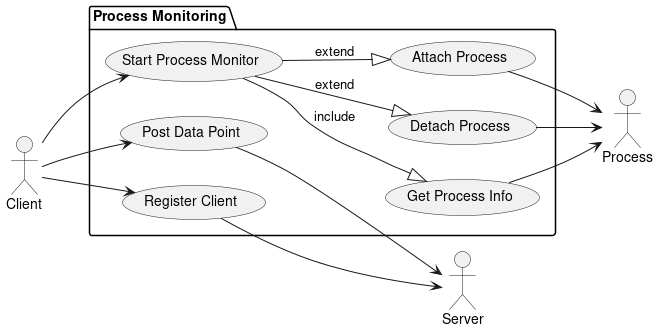
\includegraphics[scale=.7]{client.png}
\caption{Use case diagram for Client}
\centering
\end{figure}

\begin{figure}[H]
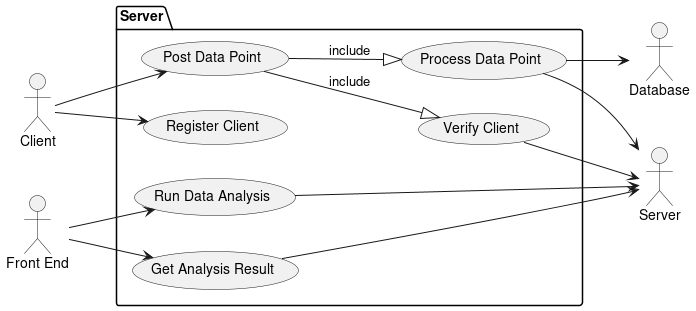
\includegraphics[scale=.7]{server.png}
\caption{Use case diagram for Server }
\centering
\end{figure}

\subsection{Class Diagrams}


\begin{figure}[H]
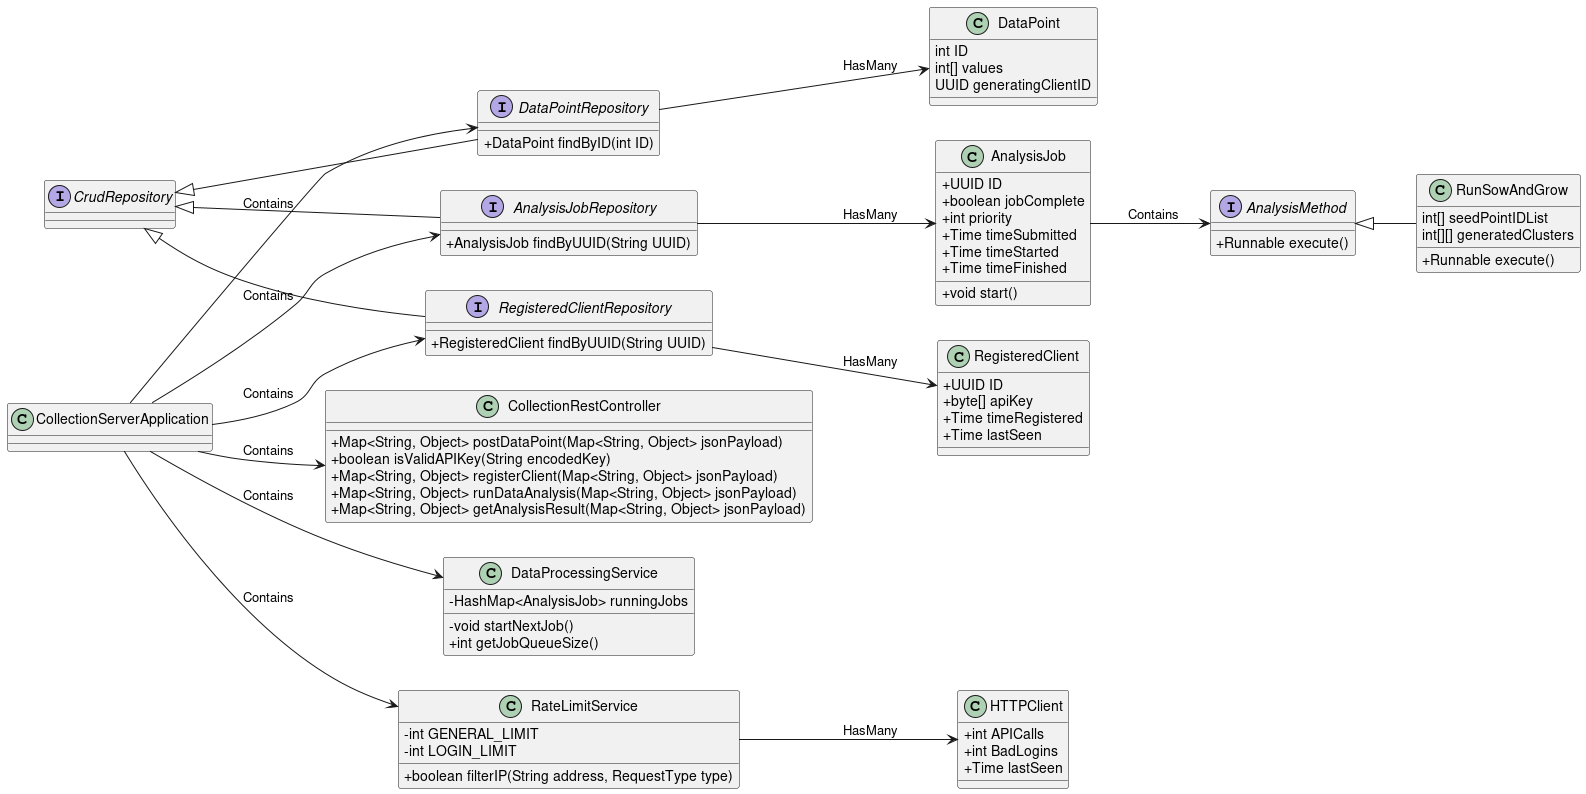
\includegraphics[scale=.325]{classDiagrams/server.png}
\caption{Class diagram for Server}

\end{figure}

\begin{figure}[H]
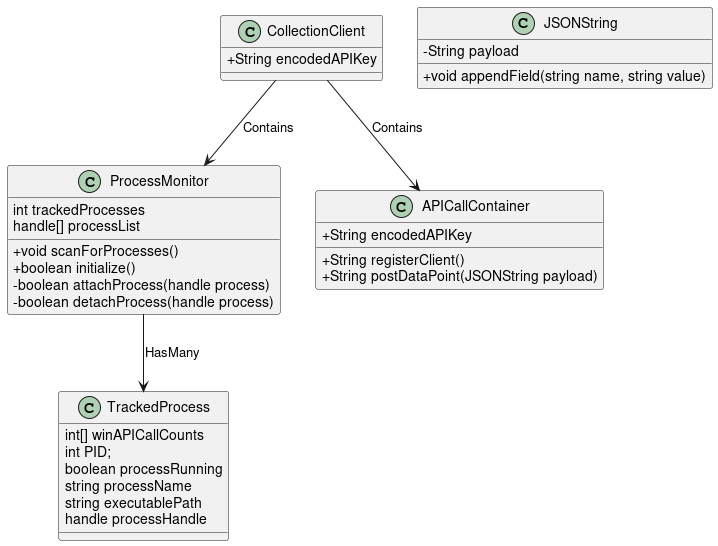
\includegraphics[scale=.6]{classDiagrams/client.png}
\caption{Class diagram for Client}
\centering
\end{figure}

\subsection{Sequence Diagrams}

\begin{figure}[H]
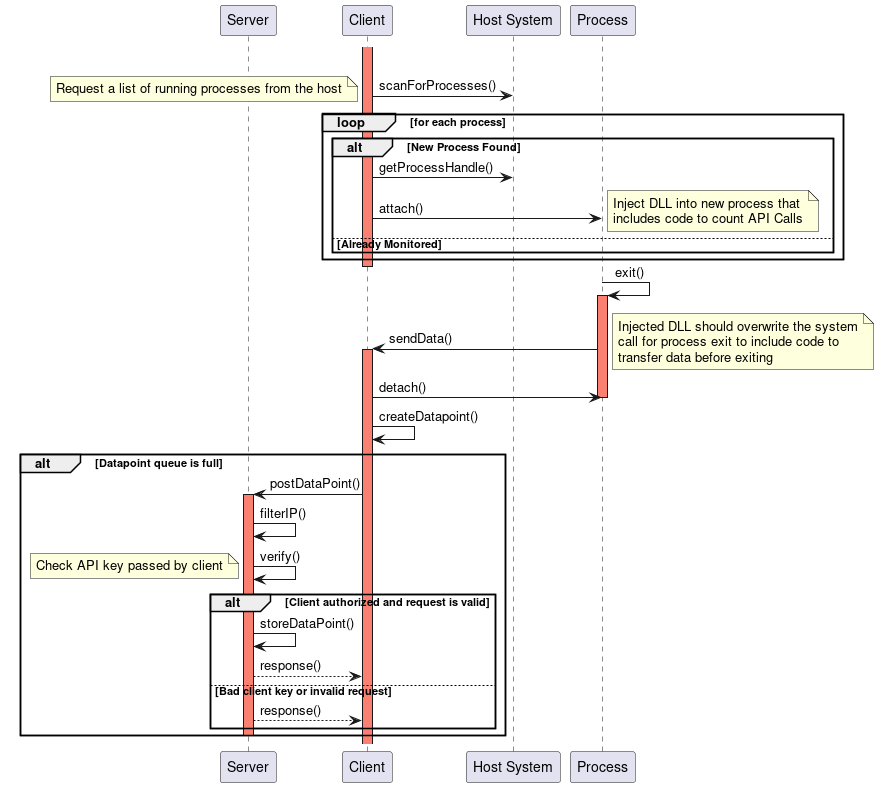
\includegraphics[scale=.57]{SequenceDiagrams/monitoringSD.png}
\caption{Sequence diagram for data collection}
\centering
\end{figure}

\section{Architecture}

\subsection{Architecture Diagram}

\begin{figure}[H]
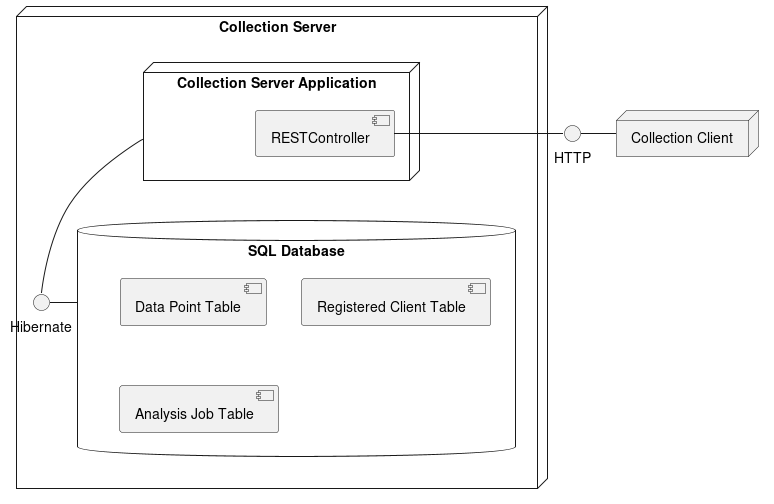
\includegraphics[scale=.57]{Architecture/arch.png}
\caption{Drawing of system architecture}
\centering
\end{figure}

\subsection{Architecture Description}
\begin{flushleft}
The system uses a Client-Server architecture. This architecture fit best since the system needs to service an arbitrary number of clients running the client software. The server will also implement a REST API to handle requests from the client software and the front end web page. The database will also not be exposed to the client or web front end. Any operations on the database will have to be done through API calls to the server.
\end{flushleft}

\section{Conclusion}
\begin{flushleft}
    I have previous experience in developing back end servers and deploying them. The main technical challenge with this project will likely be the client software. This is my first time doing Windows development. I have made some progress with an early prototype of the client software but there are several topics I will need to read into including Windows threads, DLL files, and Windows process message passing. The main motivation of this project is to create an interesting high-dimensional data set to test the Sow and Grow algorithm with, but if the system is able to consistently identify malware it could have more practical applications.
\end{flushleft}


\section{References}
\printbibliography[heading=none]


\end{document}
